\documentclass{beamer}

\usetheme{Warsaw}
\usefonttheme{professionalfonts}
%\logo{\includegraphics[height=1cm]{./images/logo.png}}
\beamertemplatenavigationsymbolsempty
\setbeamertemplate{caption}{\raggedright\insertcaption\par}
\usepackage{amsmath}
\usepackage{amssymb}
\usepackage[spanish]{babel}
\usepackage{changepage}
\usepackage{fancyvrb}
\usepackage{float}
\usepackage{framed}
\usepackage[T1]{fontenc}
\usepackage{geometry}
\usepackage{graphicx}
\usepackage{hyperref}
\usepackage[utf8]{inputenc}
\usepackage{minted}
\usepackage{multicol}
\usepackage{relsize}
\usepackage{subcaption}
\usepackage{textcomp}
\usepackage{tikz}
\usepackage{upgreek}
\usepackage{verbatim}
\usepackage{wasysym}
\usepackage{xcolor}
\definecolor{LightGray}{gray}{0.9}

%\setbeamertemplate{footline}[frame number]

\begin{document}

\title[Lógica proposicional]{Teoría de la Computación \\ Unidad 1: Lógica
  proposicional (parte 2)} \author[Teoría de la
Computación]{cristobal.loyola@usach.cl} \date{}

\titlegraphic{
  \vspace{-1.5cm}
  \begin{figure}
    \centering
    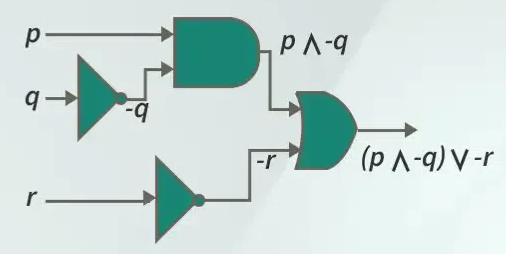
\includegraphics[width=.75\linewidth]{images/circuito_logico.png}
    \caption*{Diapositivas basadas en el material del profesor Daniel Vega}
  \end{figure}
}

\frame{\titlepage}

\setbeamertemplate{footline}[frame number]

\begin{frame}{Contenidos}

  \begin{itemize}
    \item Lógica proposicional: sintaxis (fórmula bien formada, inducción
          estructural).
    \item Semántica: valuaciones, tablas de verdad.
    \item Deducción e inferencia: método de resolución.
  \end{itemize}

\end{frame}


\begin{frame}[plain,c]
  % \frametitle{A first slide}
  \vspace{1cm}
  \begin{center}
    \Huge Sintaxis
  \end{center}
\end{frame}


\begin{frame}{Lógica proposicional: Sintaxis}
  Definiremos un conjunto de símbolos (alfabeto) dado por:
  \begin{itemize}[<+->]
    \item Un conjunto P (posiblemente infinito) de variables proposicionales: $p$, $q$, $r$, $s$,...
    \item Constantes: V o F (1 o 0, T o F)
    \item Conectores lógicos: $\sim$, $\land$, $\vee$, $\rightarrow$,
          $\leftrightarrow$
    \item Símbolos de puntuación: (, )
  \end{itemize}
\end{frame}


\begin{frame}{Lógica proposicional: Sintaxis}
  A partir de un conjunto fijo P de variables, es posible definir un lenguaje
  proposicional L(P), que contiene todas las fórmulas posibles a través de una
  definición inductiva.\\

  Así, L(P) está formado por fórmulas, donde una fórmula es:
  \begin{itemize}
    \item Una constante o un elemento de P (fórmulas atómicas).
    \item Si $\upvarphi$ es una fórmula, entonces $\sim \upvarphi$ también es
          una fórmula.
    \item Si $\upvarphi$ y $\Uppsi$ son fórmulas, entonces
          ($\upvarphi \star \Uppsi$) es una fórmula ($\star$ representa
          cualquier conector binario).
  \end{itemize}

  \textbf{Definición:} en lógica proposicional, una fórmula bien formada (FBF)
  es aquella que es obtenida usando únicamente las reglas de construcción antes
  definidas una cantidad finita de veces.
\end{frame}


\begin{frame}{Lógica proposicional: Sintaxis}
  Definiciones inductivas, como la anterior, son muy frecuentes, tanto que se
  suelen definir empleando una gramática en Backus Naur Form (BNF). En esa
  forma, la definición anterior se lee de manera más compacta como:

  $$\upvarphi ::= p \,|\, (\sim \upvarphi) \,|\, (\upvarphi \land \upvarphi) \,|\,  (\upvarphi \vee \upvarphi) \,|\,  (\upvarphi \rightarrow \upvarphi) \,|\,  (\upvarphi \leftrightarrow \upvarphi)$$

  donde $p$ representa cualquier proposición atómica y cualquier ocurrencia de
  $\upvarphi$ a la derecha de ::= representa cualquier fórmula antes construida.
\end{frame}


\begin{frame}{Lógica proposicional: Sintaxis}
  ¿Son las siguientes expresiones FBF?
  \begin{itemize}
    \item $(p \vee q) \land q$
    \item $(p \land \sim q \sim) \land \vee r)$
  \end{itemize}
\end{frame}


\begin{frame}[plain,c]
  % \frametitle{A first slide}
  \vspace{1cm}
  \begin{center}
    \Huge Inducción
  \end{center}
\end{frame}


\begin{frame}{Lógica proposicional: Inducción}
  \begin{itemize}[<+->]
    \item Sumemos los primeros 10 números naturales.
    \item Ahora, los 100 primeros naturales.
    \item ¿Y si queremos la suma de los 1000 primeros naturales?
    \item Se puede demostrar mediante inducción que:
    $$1 + 2 + 3 + ... + n = \dfrac{n (n+1)}{2}$$
  \end{itemize}
\end{frame}


\begin{frame}{Lógica proposicional: Inducción}
  La inducción matemática nos permite probar que determinada propiedad es
  satisfecha por cualquier número natural. Por ejemplo, para el caso anterior,
  basta definir $M(k)$ para indicar que la propiedad es satisfecha por $k$. Así,
  supongamos que conocemos las siguientes propiedades para $M$:\\

  \begin{itemize}
    \item \textbf{Caso base:} el número natural 1 satisface $M(1)$.
    \item \textbf{Paso inductivo:} se asume que la propiedad $M(n)$ es cierta
          para un determinado número natural $n$, luego se debe probar que para
          $n+1$ se satisface $M(n+1)$, es decir, existe una prueba de que $M(n) \rightarrow M(n+1)$.
  \end{itemize}
\end{frame}


\begin{frame}{Lógica proposicional: Inducción}
  \textbf{Definición:} sea $\upvarphi$ una FBF, definimos su altura como la suma
  entre 1 y el tamaño del camino más largo de su árbol de análisis sintáctico.\\

  Ya que cualquier FBF tiene tamaño finito, podemos mostrar declaraciones sobre
  todas las FBF por inducción matemática en sus alturas. Esta propiedad se
  conoce habitualmente como \textbf{inducción estructural}, técnica de
  razonamiento muy importante en ciencias de la computación. Por ejemplo:\\

  \textbf{Teorema:} para cada FBF, el número de paréntesis izquierdos es igual al número de paréntesis derechos.
\end{frame}


\begin{frame}{Lógica proposicional: Inducción}
  \textbf{Teorema:} para cada FBF, el número de paréntesis izquierdos es igual al número de paréntesis derechos.\\

  \textbf{Demostración:} usamos inducción sobre la altura de la FBF $\upvarphi$,
  definiendo $M(n)$ como “todas las fórmulas de altura $n$ tienen el mismo
  número de paréntesis izquierdos y derechos”. Luego, asumimos $M(k)$ para cada
  $k < n$ e intentamos probar $M(n)$.
\end{frame}


\begin{frame}{Lógica proposicional: Inducción}
  \textbf{Teorema:} para cada FBF, el número de paréntesis izquierdos es igual al número de paréntesis derechos.\\

  \textbf{Caso base (n=1):} en este caso $\upvarphi$ es una proposición atómica,
  por lo que no hay paréntesis izquierdos ni derechos, es decir, $0 = 0$.\\

  \textbf{Paso inductivo:} en este caso, el inicio del árbol sintáctico de
  $\upvarphi$ debe ser alguno de los conectores $\sim$, $\land$, $\vee$,
  $\rightarrow$ para que $\upvarphi$ sea una FBF. En particular y sin pérdida de
  generalidad, asumimos que es $\rightarrow$ (los otros casos siguen el mismo
  razonamiento). Luego, $\upvarphi$ equivale a
  $(\upvarphi_{1} \rightarrow \upvarphi_{2})$ para $\upvarphi_{1}$,
  $\upvarphi_{2}$ FBF ($\upvarphi_{1}$, $\upvarphi_{2}$ son las representaciones
  lineales de los subárboles izquierdo y derecho de $\upvarphi$). Dado que las
  alturas de $\upvarphi_{1}$ y $\upvarphi_{2}$ son estrictamente menores que
  $n$, usando la hipótesis inductiva, podemos concluir que $\upvarphi_{1}$ tiene
  el mismo número de paréntesis izquierdos y derechos, y lo mismo para
  $\upvarphi_{2}$. Pero en ($\upvarphi_{1} \rightarrow \upvarphi_{2}$) agregamos
  dos paréntesis más. Así, el número de ocurrencias de paréntesis izquierdos y
  derechos es el mismo.
\end{frame}


\begin{frame}[plain,c]
  % \frametitle{A first slide}
  \vspace{1cm}
  \begin{center}
    \Huge Semántica
  \end{center}
\end{frame}


\begin{frame}{Lógica proposicional: Semántica}
  La semántica debe proveer tres cosas:
  \begin{itemize}
    \item Significado de las fórmulas.
    \item Noción de verdad.
    \item Noción de consecuencia lógica.
  \end{itemize}
\end{frame}


\begin{frame}{Lógica proposicional: Semántica}
  \textbf{Ejemplo:} ¿cómo podemos formalizar el siguiente razonamiento?
  \[
  \begin{array}{c}
    \text{Si tomas el medicamento, te mejorarás.} \\
    \text{No estás mejorando.} \\
    \hline
    \text{Por lo tanto, no tomaste el medicamento.}
  \end{array}
  \]
\end{frame}


\begin{frame}{Lógica proposicional: Semántica}
  \textbf{Ejemplo:} ¿cómo podemos formalizar el siguiente razonamiento?
  \[
    \begin{array}{c}
      \text{Si tomas el medicamento, te mejorarás.} \\
      \text{No estás mejorando.} \\
      \hline
      \text{Por lo tanto, no tomaste el medicamento.}
    \end{array}
  \]
  \vspace{1cm}
  \[
    \begin{array}{c}
      p \rightarrow q \\
      \sim q \\
      \hline
      \sim p
    \end{array}
  \]
\end{frame}


\begin{frame}{Lógica proposicional: Semántica}
  Sea $P = \{p_{1}, p_{2}, ...\}$ un conjunto de proposiciones. Una valuación o asignación de verdad es una función:
  $$\sigma: P \rightarrow \{0, 1\}$$

  \textbf{Ejemplo:} si $P = \{p,\ q\}$, la función $\sigma_{1}$ es una valuación
  definida por:
  $$\sigma_{1}(p) = 1; \quad \sigma_{1}(q) = 0$$

  ¿Cuántas funciones de valuación distintas existen para el conjunto P anterior? ¿Y para un conjunto que contiene $n$ proposiciones?
\end{frame}


\begin{frame}{Lógica proposicional: Semántica}
  Debemos extender $\sigma$ a todo el lenguaje $L(P)$, es decir, a todas las
  posibles FBF. Sea $\upvarphi$ una fórmula proposicional, entonces:

  \begin{itemize}[<+->]
    \item Si $\upvarphi$ está en P, entonces $\sigma(\upvarphi) \in \{0, 1\}$
    \item Si $\upvarphi = V$, entonces $\sigma(\upvarphi) = 1$
    \item Si $\upvarphi = F$, entonces $\sigma(\upvarphi) = 0$
    \item Si $\upvarphi = \sim \Uppsi$, entonces
          $\sigma(\upvarphi) = 1 - \sigma(\Uppsi)$
    \item Si $\upvarphi = \Uppsi \land \upchi$, entonces
          $\sigma(\upvarphi) = \min(\sigma(\Uppsi), \sigma(\upchi))$
    \item Si $\upvarphi = \Uppsi \vee \upchi$, entonces
          $\sigma(\upvarphi) = \max(\sigma(\Uppsi), \sigma(\upchi))$
    \item Si $\upvarphi = \Uppsi \rightarrow \upchi$, entonces:
          \begin{itemize}
            \item si $\sigma(\Uppsi) = 0$ entonces $\sigma(\upvarphi) = 1$
            \item en caso contrario, $\sigma(\upvarphi) = \sigma(\upchi)$
          \end{itemize}
    \item Si $\upvarphi = \Uppsi \leftrightarrow \upchi$, entonces:
          \begin{itemize}
            \item si $\sigma(\Uppsi) = \sigma(\upchi)$ entonces
                  $\sigma(\upvarphi) = 1$
            \item en caso contrario, $\sigma(\upvarphi) = 0$
          \end{itemize}
  \end{itemize}
\end{frame}


\begin{frame}{Lógica proposicional: Semántica}
  Lo anterior puede ser resumido en una tabla de verdad:
  \begin{figure}
    \centering
    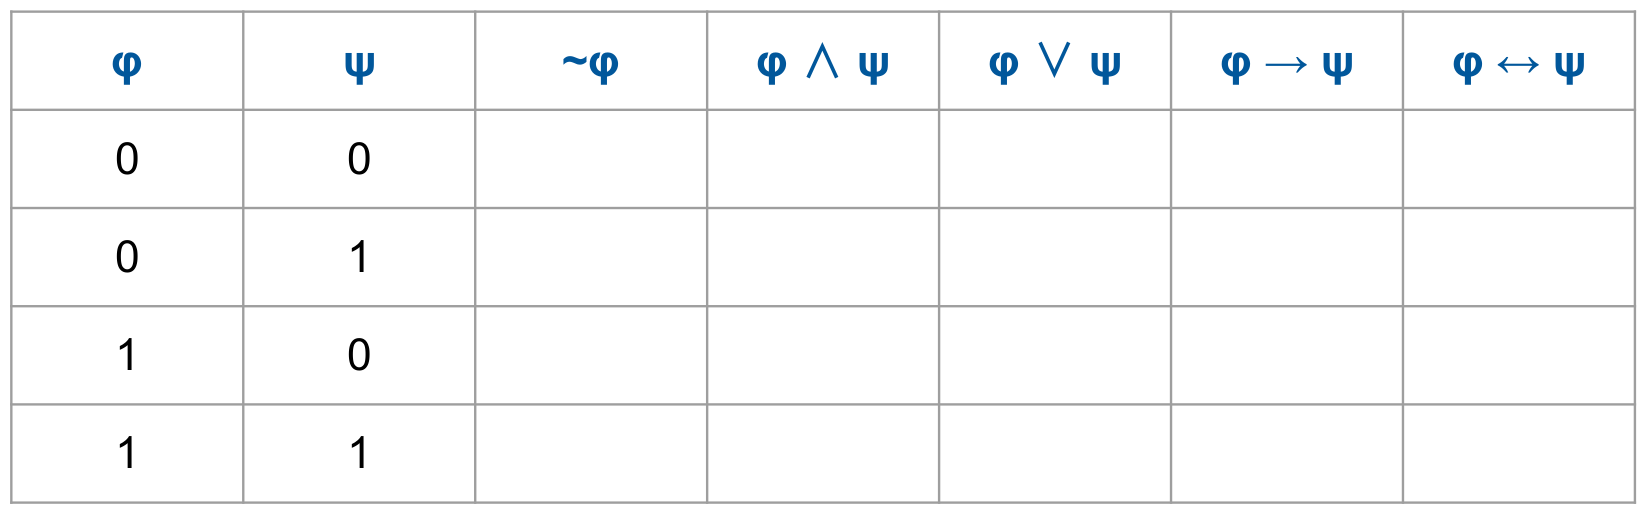
\includegraphics[width=1.\textwidth]{images/resumen_tabla_de_verdad_blanco.png}
  \end{figure}
\end{frame}


\begin{frame}{Lógica proposicional: Semántica}
  Lo anterior puede ser resumido en una tabla de verdad:
  \begin{figure}
    \centering
    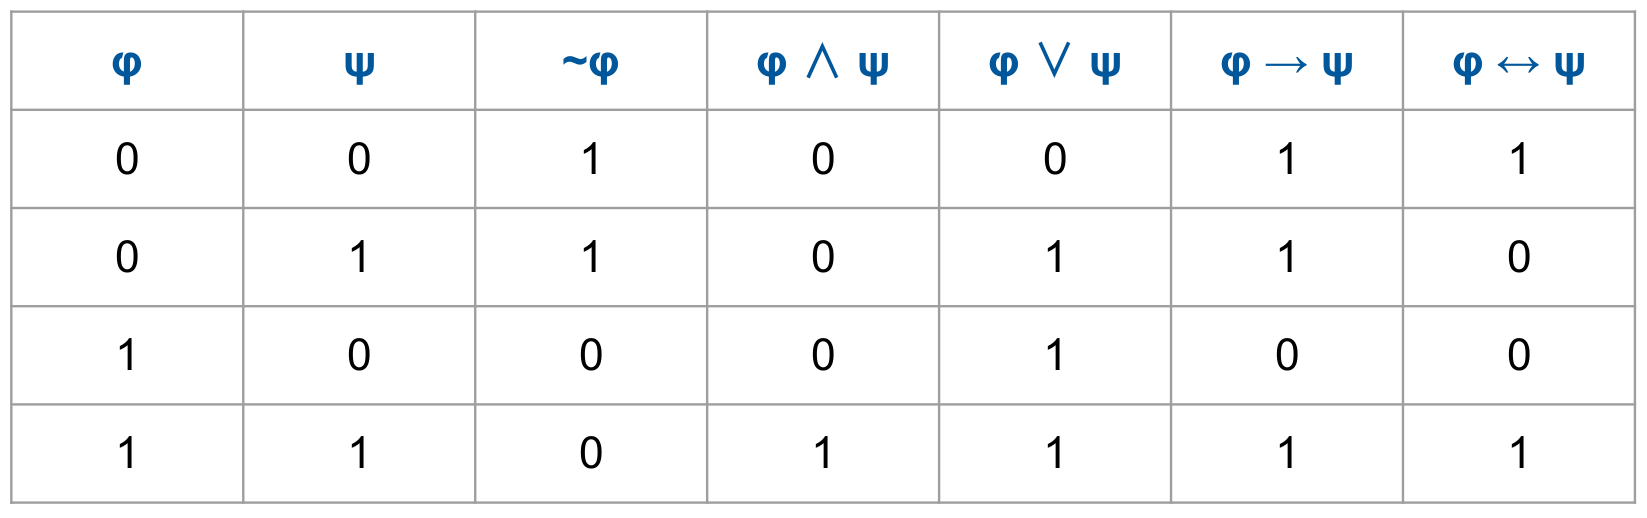
\includegraphics[width=1.\textwidth]{images/resumen_tabla_de_verdad.png}
  \end{figure}

  \textbf{Definición:} una fórmula $\Uppsi$ es \textbf{equivalente} a otra
  fórmula $\upchi$ si y sólo si $\sigma(\upvarphi) = \sigma(\upchi)$ para toda
  valuación $\sigma$ (es decir, deben tener exactamente la misma tabla de
  verdad).
\end{frame}


\begin{frame}{Lógica proposicional: Semántica}
  \textbf{Definición:} una fórmula es \textbf{satisfacible} si es verdadera para
  alguna valuación $\sigma$.\\

  \textbf{Ejemplo:} indique si la siguiente expresión es satisfacible:
  $$\sim p \land (p \vee q)$$

  \begin{figure}
    \centering
    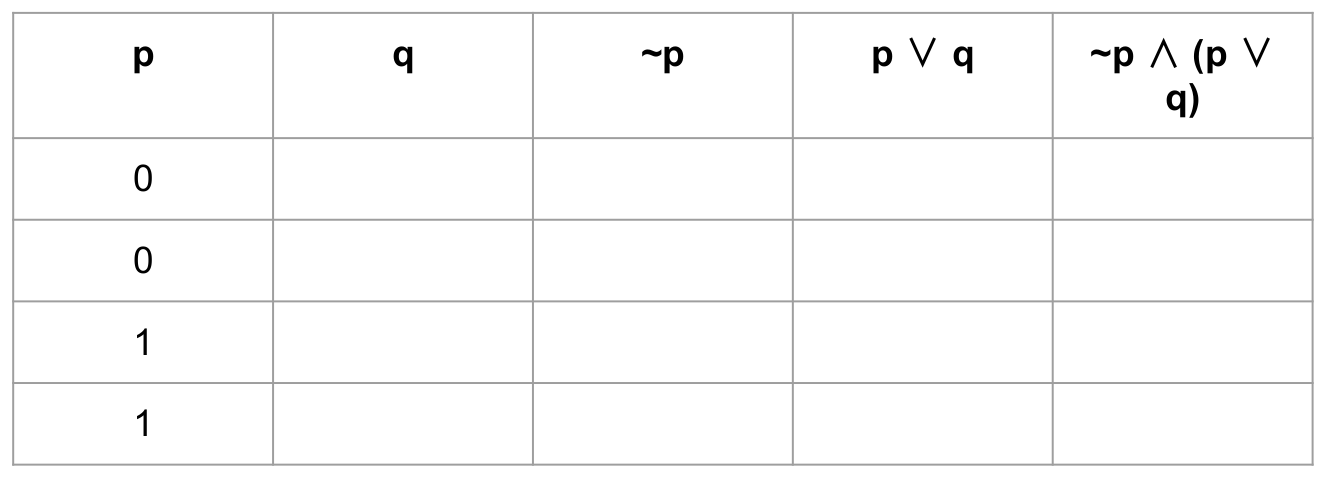
\includegraphics[width=1.\textwidth]{images/tabla_de_verdad_01_blanco.png}
  \end{figure}
\end{frame}


\begin{frame}{Lógica proposicional: Semántica}
  \textbf{Definición:} una fórmula es \textbf{satisfacible} si es verdadera para
  alguna valuación $\sigma$.\\

  \textbf{Ejemplo:} indique si la siguiente expresión es satisfacible:
  $$\sim p \land (p \vee q)$$

  \begin{figure}
    \centering
    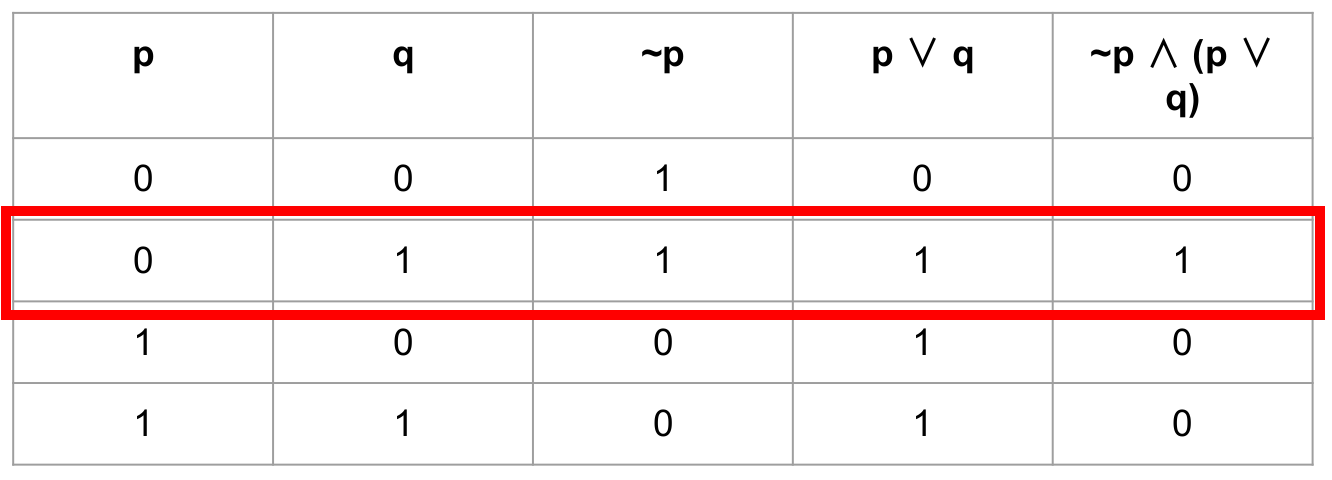
\includegraphics[width=1.\textwidth]{images/tabla_de_verdad_01_rojo.png}
  \end{figure}
\end{frame}


\begin{frame}{Lógica proposicional: Semántica}
  \textbf{Definición:} un conjunto de fórmulas $\Sigma$ es satisfacible
  \textbf{si existe al menos una valuación} $\sigma$ que hace verdaderas a todas
  las fórmulas de $\sigma$. Esto último se denota como:

  $$\sigma \vDash \Sigma$$

  Un conjunto de fórmulas que no se puede satisfacer (insatisfacible) se le
  conoce como \textbf{inconsistente}.
\end{frame}


\begin{frame}{Lógica proposicional: Semántica}
  \begin{itemize}[<+->]
    \item Si una fórmula es verdadera para toda valuación $\sigma$, entonces
          diremos que es una \textbf{tautología}.
          \begin{itemize}
            \item \textbf{Ej:} $p \vee \sim p$
          \end{itemize}

    \item Si una fórmula es falsa para toda valuación $\sigma$, entonces diremos
          que es una \textbf{contradicción}.
          \begin{itemize}
            \item \textbf{Ej:} $p \land \sim p$
          \end{itemize}

    \item Si una fórmula es verdadera para al menos una valuación $\sigma_{1}$ y
          falsa para al menos otra valuación $\sigma_{2}$, entonces diremos que
          es una \textbf{contingencia}.
          \begin{itemize}
            \item \textbf{Ej:} $p \vee q$
          \end{itemize}
  \end{itemize}
\end{frame}


\begin{frame}{Lógica proposicional: Semántica}
  \textbf{Ejercicio:} formalice el siguiente razonamiento y determine si es una tautología, una contradicción o una contingencia:
  \[
    \begin{array}{c}
      \text{Si toma el medicamento, se recuperará.} \\
      \text{Usted no está tomando el medicamente} \\
      \hline
      \text{Por lo tanto, usted no se recuperará.}
    \end{array}
  \]
\end{frame}


\begin{frame}{Lógica proposicional: Semántica}
  \textbf{Ejercicio:} determine si las siguientes fórmulas corresponden a una
  tautología, una contradicción o una contingencia.

  \begin{enumerate}
    \item $p \rightarrow (q \rightarrow p)$
    \item $(p \leftrightarrow q) \vee q$
    \item $(p \rightarrow q) \rightarrow (\sim(q \rightarrow p))$
    \item $\sim(((p \rightarrow q) \rightarrow p) \rightarrow p)$
  \end{enumerate}
\end{frame}


\begin{frame}[plain,c]
  % \frametitle{A first slide}
  \vspace{1cm}
  \begin{center}
    \Huge Deducción
  \end{center}
\end{frame}


\begin{frame}{Lógica proposicional: Deducción}
  \textbf{Definición:} un conjunto $C$ de conectores lógicos es
  \textbf{funcionalmente completo} si es posible definir a todos los conectores
  estándar en función de los que contiene C.

  Por ejemplo, el conjunto:

  $$ C = \{\sim,\ \vee,\ \land\}$$

  es funcionalmente completo.\\

  ¿Es posible encontrar un conjunto $C'$ aún más pequeño?
\end{frame}


\begin{frame}{Lógica proposicional: Deducción}
  Las formas normales son formas sintácticas estándares que pueden cumplir las
  fórmulas.\\

  Por ejemplo:
  \begin{itemize}
    \item Forma Normal Conjuntiva (\textbf{FNC})
    \item Forma Normal Disyuntiva (\textbf{FND})
  \end{itemize}
\end{frame}


\begin{frame}{Lógica proposicional: Deducción}
  \begin{itemize}[<+->]
    \item \textbf{Definición:} un \textbf{literal} es una variable
          proposicional, o una variable proposicional negada o una constante V o
          F.
    \item \textbf{Definición:} una \textbf{cláusula} es una disyunción de
          literales, es decir, es de la forma:
          $$I_{1} \vee I_{2} \vee I_{3} \vee ... \vee I_{k}$$
    \item \textbf{Definición:} una \textbf{cláusula dual} es una conjunción de
          literales, es decir, es de la forma:
          $$I_{1} \land I_{2} \land I_{3} \land ... \land I_{k}$$
  \end{itemize}
\end{frame}


\begin{frame}{Lógica proposicional: Deducción}
  \textbf{Definición:} una fórmula en \textbf{Forma Normal Conjuntiva} (FNC) es
  una \textbf{conjunción} de cláusulas. Si cada $c_{i}$ es una cláusula,
  entonces la FNC es de la forma:

  $$c_{1} \land c_{2} \land c_{3} \land ... \land c_{n}$$

  Por ejemplo, la siguiente fórmula está en FNC:
  $$(p \vee \sim q \vee s) \land (p \vee s) \land p$$
\end{frame}


\begin{frame}{Lógica proposicional: Deducción}
  \textbf{Definición:} una fórmula en \textbf{Forma Normal Disyuntiva} (FND) es
  una \textbf{disyunción} de cláusulas duales. Si cada $c^{'}_{i}$ es una
  cláusula dual, entonces la FND es de la forma:

  $$c^{'}_{1} \vee c^{'}_{2} \land c^{'}_{3} \land ... \land c^{'}_{n}$$

  Por ejemplo, la siguiente fórmula está en FND:
  $$(p \land q) \vee q \vee (\sim p \land s)$$
\end{frame}


\begin{frame}{Lógica proposicional: Deducción}
  \textbf{Teorema:} Toda fórmula es equivalente a una fórmula en FNC.

  \vspace{1cm}

  \textbf{Teorema:} Toda fórmula es equivalente a una fórmula en FND.
\end{frame}


\begin{frame}{Lógica proposicional: Deducción}
  \textbf{Definición:} una inferencia es \textbf{válida} si y sólo si en todos
  los casos en los que todas las premisas son verdaderas, la conclusión también
  es verdadera.

  \[
    \begin{array}{c}
      \upvarphi_{1}, ..., \upvarphi_{n}\\
      \hline
      \Uppsi
    \end{array}
  \]

  Lo anterior se puede denotar equivalentemente como:
  \begin{itemize}
    \item $\Uppsi$ es una consecuencia lógica de
          $\Sigma = \{\upvarphi_{1}, ..., \upvarphi_{n}\}$
    \item $\upvarphi_{1}, ..., \upvarphi_{n} \vDash \Uppsi$
    \item $\Sigma \vDash \Uppsi$
  \end{itemize}
\end{frame}


\begin{frame}{Lógica proposicional: Deducción}
  Una lógica se considera \textbf{monótona} si a medida que se agregan fórmulas
  a una base de conocimiento, los hechos que se concluyan a partir de la base
  original siguen siendo válidos.\\

  Formalmente, sean $\Sigma_{1}$ y $\Sigma_{2}$ dos conjuntos de fórmulas tales que $\Sigma_{1} \subseteq \Sigma_{2}$, entonces:

  $$\text{Si } \Sigma_{1} \vDash \upvarphi \text{, entonces } \Sigma_{2} \vDash \upvarphi$$

  En otras palabras, si una conclusión se puede inferir de un conjunto de
  premisas, entonces esa conclusión seguirá siendo válida incluso si se añaden
  más premisas.
\end{frame}


\begin{frame}{Lógica proposicional: Deducción}
  \textbf{Regla de resolución:} supongamos que tenemos la siguiente fórmula en
  FNC:
  $$(p \vee q\ \vee \sim r) \land (\sim q \vee s\ \vee \sim t)$$

  y que $\sigma$ es una valuación que la hacer verdadera. Entonces, podemos distinguir dos casos:

  \begin{itemize}
    \item Si $\sigma \vDash q$, entonces $\sigma \vDash s\ \vee \sim t$
    \item Si $\sigma \nvDash q$, entonces $\sigma \vDash p\ \vee \sim r$
  \end{itemize}

  Por lo tanto, podemos concluir que
  $\sigma \vDash (p\ \vee \sim r \vee s\ \vee \sim t)$\\

  (Note que hemos conseguido eliminar un literal y su negado, para obtener una
  cláusula con una proposición menos)
\end{frame}


\begin{frame}{Lógica proposicional: Deducción}
  \textbf{Teorema de deducción:} sea $\Sigma \subseteq L(P)$, entonces:

  $$\Sigma \vDash (\upvarphi \rightarrow \Uppsi) \text{ si y sólo si } \Sigma \cup \{\upvarphi\} \vDash \Uppsi$$
\end{frame}


\begin{frame}{Lógica proposicional: Deducción}
  \textbf{Demostración por resolución (DPR):} está basado en la reducción entre
  consistencia y consecuencia lógica. Supongamos que queremos demostrar que
  $\Sigma \vDash \upvarphi$:

  $$\Sigma \vDash \upvarphi \Leftrightarrow \Sigma \cup \{\sim \upvarphi\} \text{ es inconsistente }$$

  El lado derecho de la equivalencia es lo mismo que $\Sigma \vDash \square$,
  donde el símbolo $\square$ corresponde a la cláusula vacía (sin literales, y
  por lo tanto no satisfacible).
\end{frame}


\begin{frame}{Lógica proposicional: Deducción}
  \textbf{Demostración por resolución:} para demostrar que
  $\Sigma \vDash \Uppsi$ seguiremos los siguientes pasos:

  \begin{itemize}
    \item Transformar $\Sigma \cup \{\sim \Uppsi\}$ a FNC, con un conjunto de
          cláusulas $C = \{C_{1}, ..., C_{n}\}$
    \item Mientras $\square \notin C$ y existan $C_{i}, C_{j} \in C$ para
          aplicar la regla de resolución:
          \begin{itemize}
            \item Aplicar regla de resolución $C_{i}, C_{j}$, generando $C'$.
            \item Hacer $C := C \cup \{C'\}$
          \end{itemize}
  \end{itemize}

  Si $\square \in C$, entonces $\Sigma \vDash \Uppsi$
\end{frame}


\begin{frame}{Lógica proposicional: Deducción}
  \textbf{Ejercicio:} sea $\Sigma = \{p,\ q \rightarrow (p \rightarrow r)\}$.
  Utilice la demostración por resolución para comprobar que
  $\Sigma \vDash (q \rightarrow r)$
\end{frame}


\begin{frame}{Lógica proposicional: Deducción}
  \textbf{Ejercicio:} sea $\Sigma = \{p,\ q \rightarrow (p \rightarrow r)\}$.
  Utilice la demostración por resolución para comprobar que
  $\Sigma \vDash (q \rightarrow r)$

  \begin{figure}
    \centering
    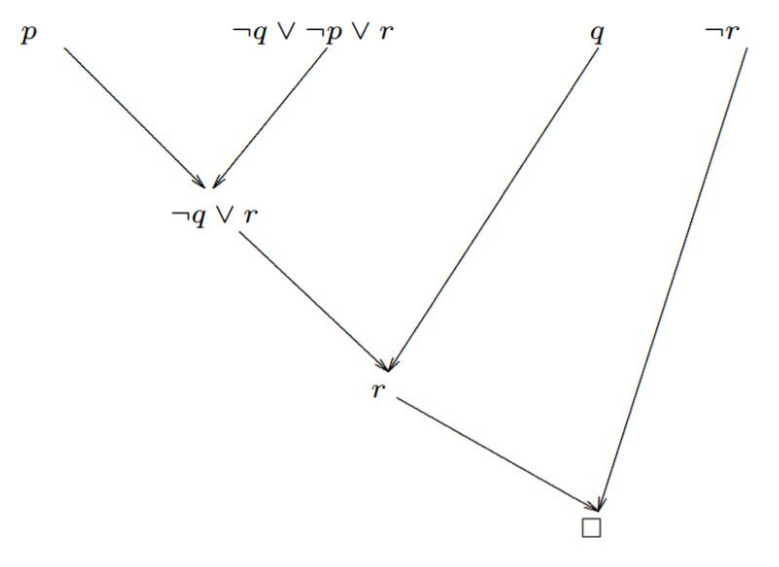
\includegraphics[width=.8\textwidth]{images/demostracion_por_resolucion.png}
  \end{figure}
\end{frame}


\begin{frame}{Lógica proposicional: Deducción}
  \textbf{Ejercicio:} sea $\Sigma = \{p,\ q \rightarrow (p \rightarrow r)\}$.
  Utilice la demostración por resolución para comprobar que
  $\Sigma \vDash (q \rightarrow r)$

  \begin{figure}
    \centering
    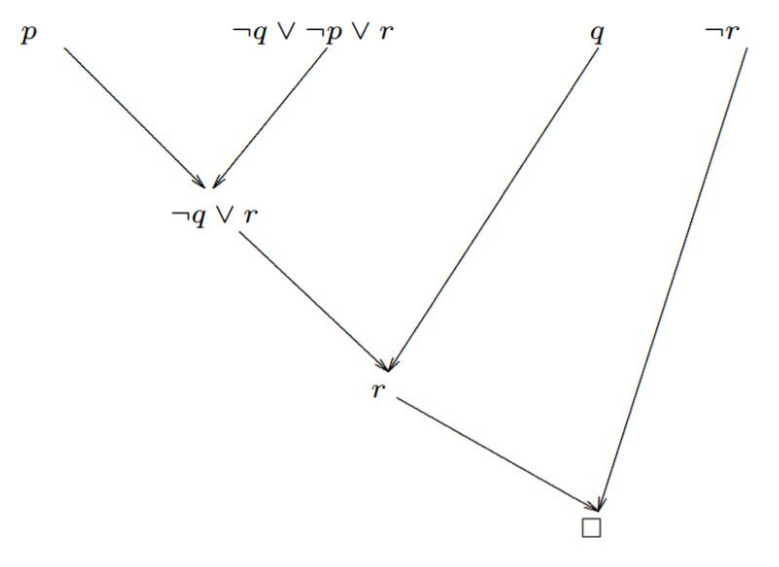
\includegraphics[width=.8\textwidth]{images/demostracion_por_resolucion.png}
  \end{figure}
\end{frame}


\begin{frame}{Lógica proposicional: Deducción}
  \begin{itemize}
    \item Una \textbf{demostración} es una secuencia finita de fórmulas
          (válidas) en la cual cada fórmula es un axioma, o bien ha sido
          derivada a partir de fórmulas anteriores mediante una regla de
          inferencia.
    \item Un \textbf{teorema} es una fórmula derivada de una demostración.
    \item Un \textbf{sistema axiomático} es un conjunto de axiomas y reglas de
          inferencia.
          \begin{itemize}
            \item Un sistema axiomático es correcto para una lógica dada si todo
                  teorema es válido en la lógica.
            \item Un sistema axiomático es completo para una lógica dada si toda
                  fórmula válida de la lógica es un teorema.
          \end{itemize}


  \end{itemize}
\end{frame}





\end{document}
